\documentclass{article}

\usepackage{libertine}
\usepackage[libertine]{newtxmath}

\usepackage{hyperref, amsmath, amssymb}
\usepackage{amsfonts}
\usepackage{graphics}
\usepackage{tikz}
\usepackage{graphicx}
\usepackage{enumerate}
\usepackage{color}
\usepackage{mathtools}
\usepackage{stmaryrd}

\usepackage{pgf, latexsym, float, soul, array, booktabs, dsfont, gensymb, wasysym, multicol, tcolorbox, tabularx, enumitem, multirow}

\usepackage{ marvosym }

\usepackage{enumitem}
\setlist[itemize]{leftmargin=2em, itemsep=-.25em, topsep=0em}

\newenvironment{bx}[1][]{
\begin{tcolorbox}[colback=white!97!black, title=#1, arc=0in, halign=flush left, left=1mm, right=1mm,]
}{
\end{tcolorbox}
}


\usepackage[margin=0.2in]{geometry}

% \setlength{\columnsep}{1pt}
% \setlength{\columnseprule}{1pt}

\begin{document}
% \begin{huge}
% \begin{center}
% Condensed Calculus
% \end{center}
% \end{huge}
% \noindent \hrule

\begin{center}
\setlength{\tabcolsep}{2pt}
\begin{tabular}{p{2.5in} p{5.25in}}

\begin{bx}[Trigonometry]
$(\cos\theta,\sin\theta)$ is the coordinate on the unit circle that makes angle $\theta$ with the positive $x$-axis.
$$\sec\theta=\frac{1}{\cos\theta}\quad \quad\csc\theta=\frac{1}{\sin\theta}$$
$$\tan\theta=\frac{\sin\theta}{\cos\theta}\quad \quad \cot\theta=\frac{\cos\theta}{\sin\theta}$$
$${\text{Pythagorean}\atop\text{identities}}\begin{cases}
\sin^2\theta + \cos^2\theta = 1 \\
\tan^2\theta + 1 = \sec^2\theta \\
1 + \cot^2\theta = \csc^2\theta
\end{cases}$$
$$\sin(A\pm B)=\sin A\cos B\pm\cos A\sin B$$
$$\cos(A\pm B)=\cos A\cos B\mp\sin A\sin B$$
$$\sin(2\theta)=2\sin\theta\cos\theta$$
$$\cos(2\theta) =\cos^2\theta-\sin^2\theta$$

\begin{center}
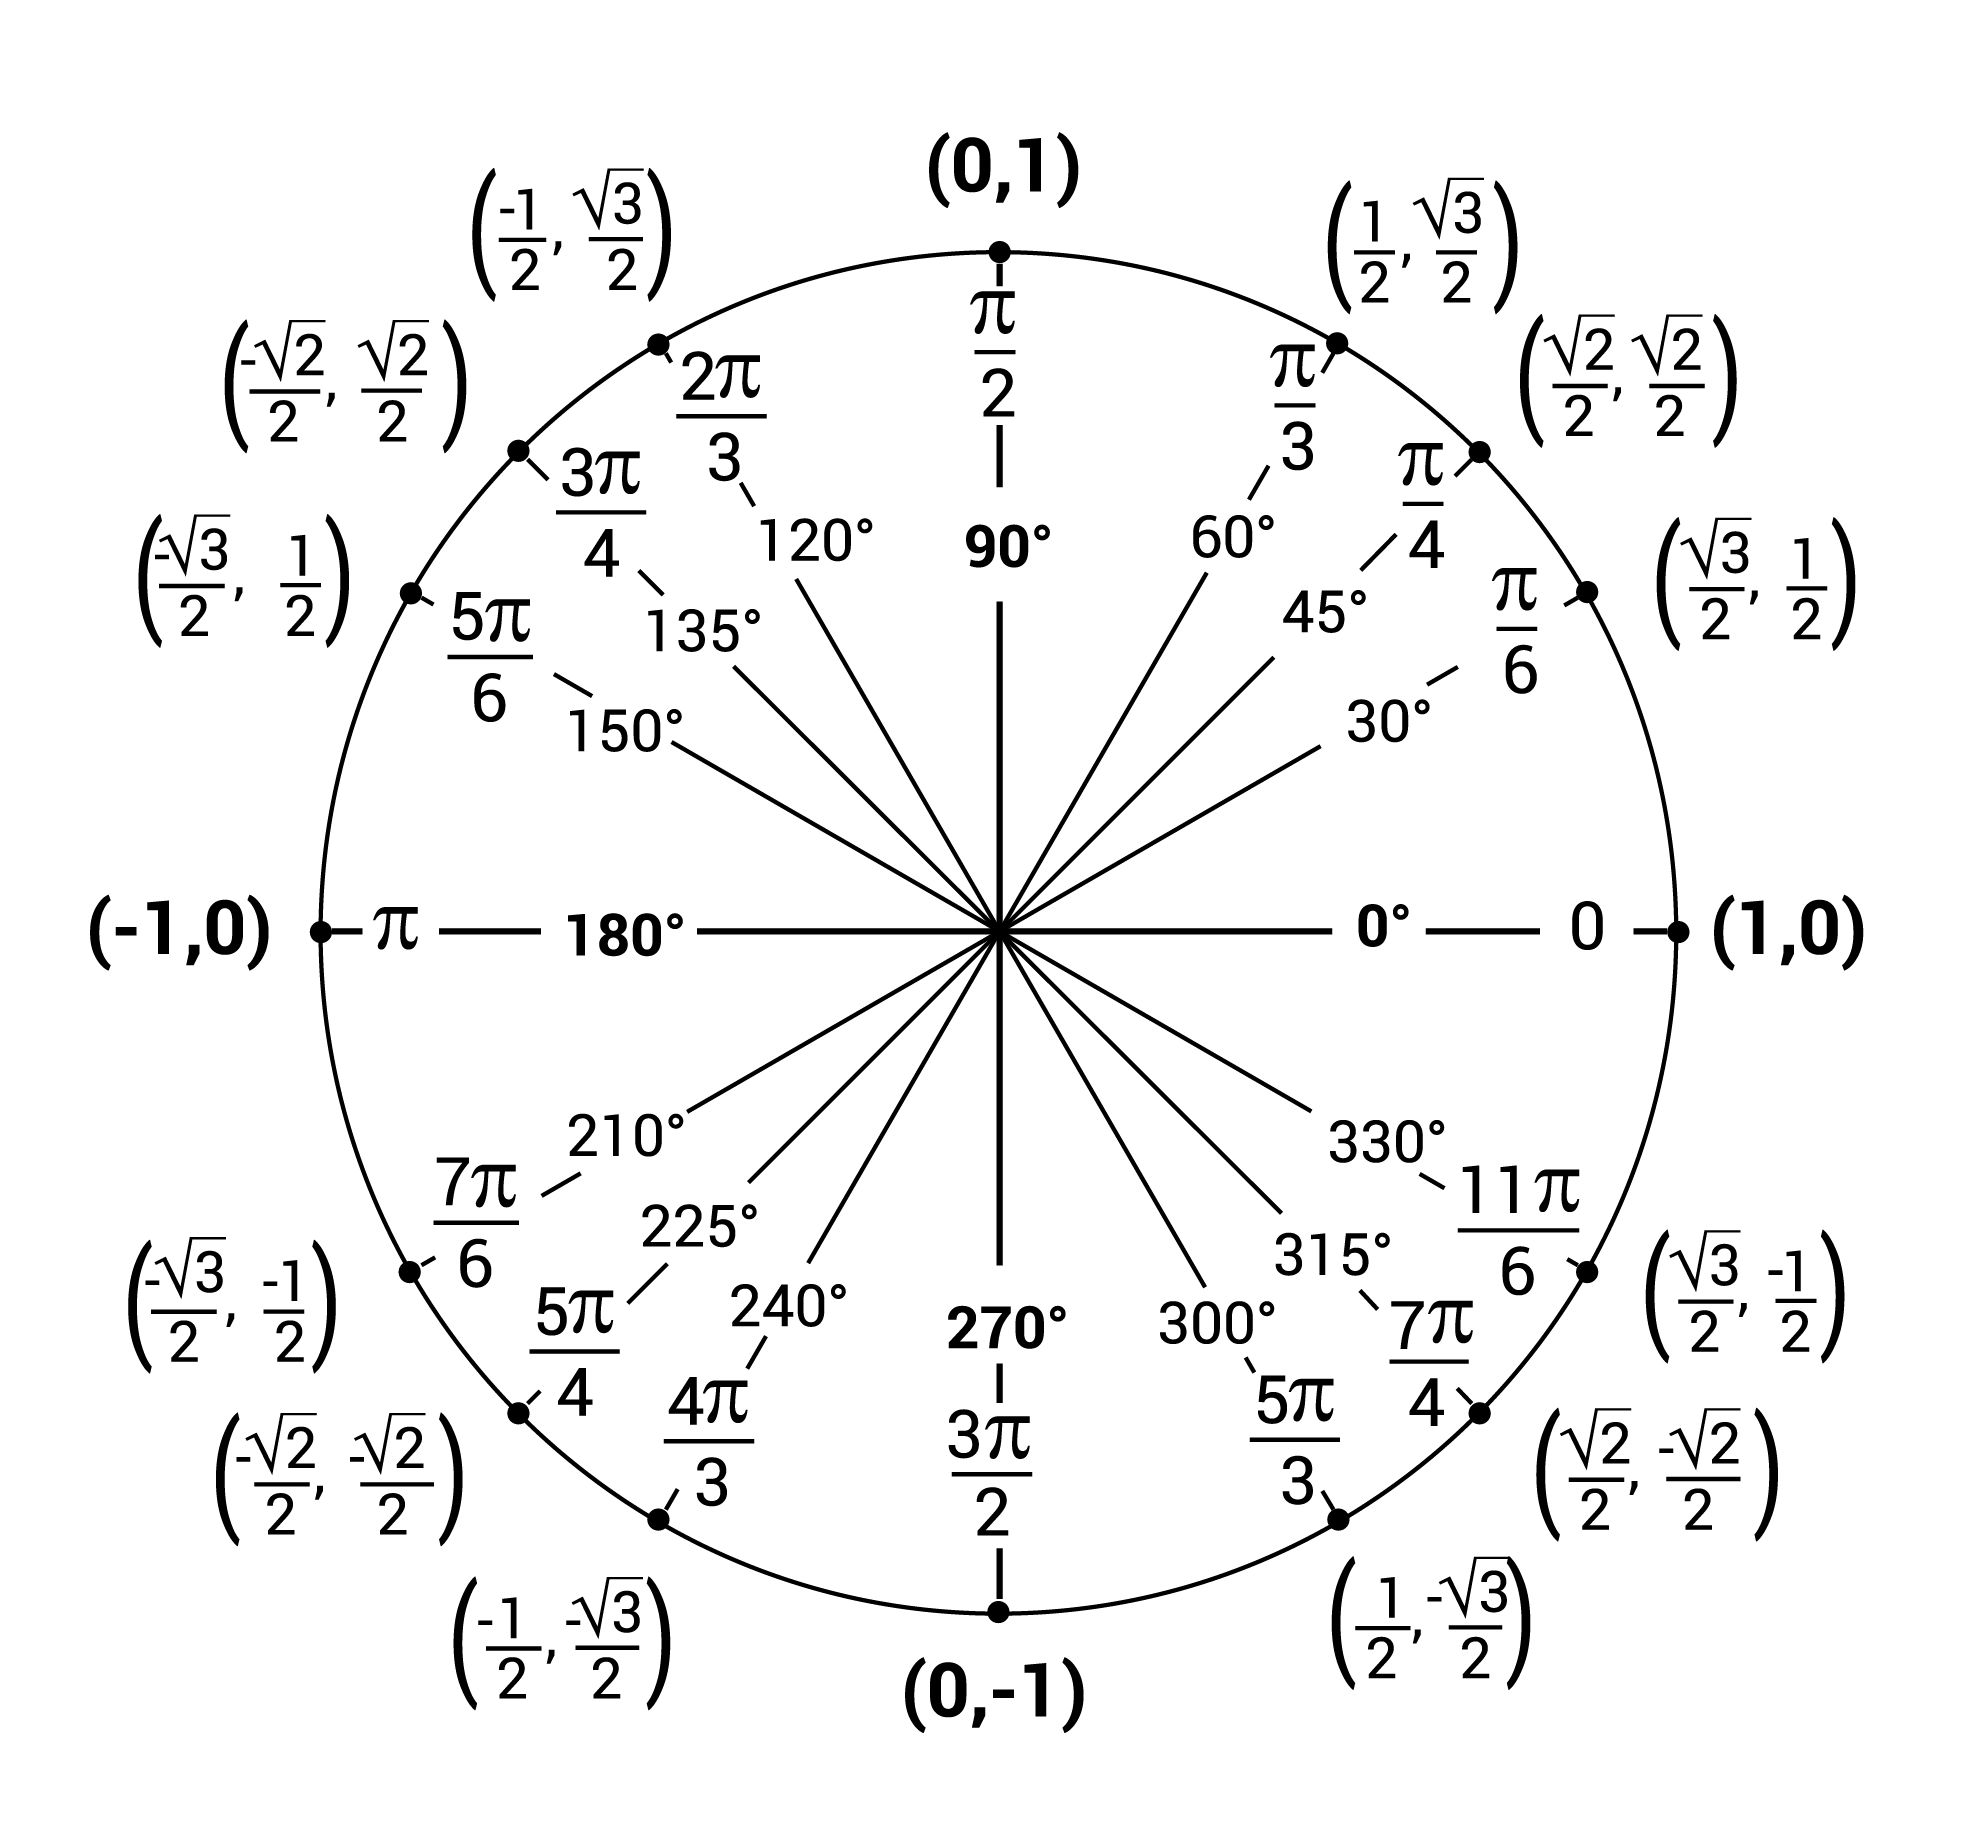
\includegraphics[width=2.3in]{img/unit-circle.png}
\end{center}
\end{bx}

&

\vspace{-5.76in}

\begin{bx}[Limits]
\begin{tabular}{p{3in} p{1.9in}}
\begin{center}

\vspace{-2em}

\def\arraystretch{1.5}
\begin{tabular}{ll}
\textbf{Law} & Let $\displaystyle \lim_{x\to a} f(x)= L$ and $\displaystyle \lim_{x\to a} g(x)= M$.\\
\toprule[0.4mm]
\textbf{Sum} & $\displaystyle\lim _{x \rightarrow a}(f(x)+g(x))=L+M$ \\
\textbf{Scalar} & $\displaystyle\lim _{x \rightarrow a} c f(x)=c L$ \\
\textbf{Product} & $\displaystyle\lim _{x \rightarrow a}(f(x) \cdot g(x))=L \cdot M$ \\
\textbf{Quotient} & $\displaystyle\lim _{x \rightarrow a} \frac{f(x)}{g(x)}=\frac{L}{M}$ for $M \neq 0$ \\
\textbf{Power} & $\displaystyle\lim _{x \rightarrow a}(f(x))^{n}=L^{n}$\\
\textbf{Root} & $\displaystyle\lim _{x \rightarrow a} \sqrt[n]{f(x)}=\sqrt[n]{L}$ for all $L$ if $n$ is odd, \\ & and for $L \geq 0$ if $n$ is even and $f(x) \geq 0 .$ \\
\bottomrule[0.4mm]
\end{tabular}
\end{center}
 &
\textbf{Squeeze Theorem:}

Let $f$, $g$, and $h$ be functions with $g(x)\leq f(x)\leq h(x)$ for all $x$ and $\displaystyle\lim_{x\to a}g(x)=L=\lim_{x\to a} h(x)$, then $\displaystyle\lim_{x\to a} f(x)=L$.

\vspace{1em}

\textbf{Indeterminate Forms:}

$\frac{0}{0}$, $\frac{\infty}{\infty}$, $0^0$, $\infty-\infty$, $1^\infty$, $0\cdot\infty$, $\infty^0$

\vspace{1em}

\textbf{$\varepsilon-\delta$ definition:}

$L$ is the limit of $f$ as $x$ approaches $a$ if for all $\varepsilon > 0$, there is some

$\delta > 0$, such that 

$|x - a| < \delta \implies |f(x) - L| <\varepsilon$.

\end{tabular}

\vspace{-0.25em}

$$\lim_{x\to 0}\frac{\sin(x)}{x} = 1\quad\quad\lim_{x\to\infty}\left(1+\frac{1}{x}\right)^x = e\quad\quad \lim_{x\to\infty}\frac{ax^n+\dots}{bx^m+\dots}=\begin{cases}0 & m>n \\ \infty & n > m \\ a/b & n=m\end{cases}$$

\end{bx}

\vspace{-0.25em}

\begin{bx}[Continuity]
\textbf{Definition:} $f$ is \textit{continuous} at $x=a$ if $\displaystyle\lim_{x\to a}f(x)=f(a)$.

\begin{itemize}
\setlength\itemsep{-0.25em}
\item The following functions are \textbf{continuous on their domains}: polynomials, rational functions, trig and inverse trig functions, exponential functions, logarithms.
\item The sum, product, and composition of continuous functions is continuous.
\end{itemize}

\vspace{0.5em}

\begin{tabular}{p{1.9in} | p{3in}}
\textbf{Composite Function Theorem}:

If $f(x)$ is continuous at $L$

and $\displaystyle\lim _{x \to a} g(x)=L$, then

$\displaystyle\lim_{x \to a} f(g(x))=f(L).$
&
\textbf{The Intermediate Value Theorem:}

Let $f$ be continuous over a closed, bounded interval $[a, b]$. If $z$ is any real number between $f(a)$ and $f(b)$, then there is a number $c$ in $[a, b]$ satisfying $f(c)=z$.
\end{tabular}

\end{bx}

\end{tabular}

\vspace{-1.25em}

\begin{tabular}{p{563pt}}
\begin{bx}[Derivatives]

\begin{tabular}{p{3in} p{4.4in}}

\textbf{Limit definition} of the derivative:
$$f'(x)=\lim_{h\to 0}\frac{f(x+h)-f(x)}{h}=\lim_{x\to a}\frac{f(x)-f(a)}{x-a}$$
\textbf{Tangent line} to $f(x)$ at $x=a$:
$$L(x)=f(a) + f'(a)(x-a)$$

\textbf{L'H\^opital's Rule:}

If $\displaystyle \lim_{x\to a} f(x)= \lim_{x\to a} g(x)= 0$ or $\infty$, then
$$\lim_{x\to a}\frac{f(x)}{g(x)}=\lim_{x\to a}\frac{f'(x)}{g'(x)}.$$

\vspace{0.25em}

\begin{center}
\def\arraystretch{1.5}
\begin{tabular}{ll}
\toprule[0.4mm]
\textbf{The Scalar Rule} & $[af]' = af'$ \\
\textbf{The Sum Rule} & $[f + g]' = f' + g'$ \\
\textbf{The Product Rule} & $[fg]' = f'g + fg'$ \\
\textbf{The Quotient Rule} & $\left[\frac{f}{g}\right]' = \frac{f'g - fg'}{g^2}$ \\
\textbf{The Chain Rule} & $[f(g(x))]' = f'(g(x))g'(x)$ \\
\textbf{The Inverse Rule} & $[f^{-1}(x)]' = \frac{1}{f'(f^{-1}(x))}$ \\
\bottomrule[0.4mm]
\end{tabular}
\end{center}

&

% \vspace{2em}

\textbf{Logarithmic Differentiation:}

To find the derivative of $y=f(x)^{g(x)}$, take $\ln()$ of both sides, bring $g(x)$ down using the log rule ($\ln(a^b)=b\ln(a)$):
$$\ln(y)=\ln(f(x)^g(x))=g(x)\ln(f(x))$$
Then implicitly differentiate and solve for $y'$:
$$y'=f(x)^{g(x)}\left(g'(x)\ln(f(x))+g(x)\frac{f'(x)}{f(x)}\right).$$


\begin{center}
\def\arraystretch{1.5}
\begin{tabular}{lll}
\toprule[0.4mm]
\textbf{The Power Rule}        & $[x^a]' = ax^{a-1}$ \\
\textbf{Trig Rules}  & $[\sin(x)]' = \cos(x)$ & $[\cos(x)]' = -\sin(x)$ \\
(PSST!)& $[\tan(x)]'=\sec^2(x)$ & $[\cot(x)]'=-\csc^2(x)$\\
& $[\sec(x)]'=\sec(x)\tan(x)$ & $[\csc(x)]'=-\csc(x)\cot(x)$ \\
\textbf{Inverse Trig Rules} & $[\sin^{-1}(x)]'=\frac{1}{\sqrt{1-x^2}}$ & $[\cos^{-1}(x)]'=\frac{-1}{\sqrt{1-x^2}}$\\

& $[\csc^{-1}(x)]'=\frac{-1}{|x|\sqrt{x^2-1}}$ & $[\sec^{-1}(x)]'=\frac{1}{|x|\sqrt{x^2-1}}$ \\
& $[\tan^{-1}(x)]'=\frac{1}{1+x^2}$ & $[\cot^{-1}(x)]'=\frac{1}{1+x^2}$\\
\textbf{Exponent Rule} & $[a^x]' = \ln(a)a^x$ \\
\textbf{Logarithm Rule} & $[\log_a(x)]' = \frac{1}{x\ln(a)}$ \\
\bottomrule[0.4mm]
\end{tabular}
\end{center}

\end{tabular}


\end{bx}
\end{tabular}





\end{center}




\end{document}
